%% BenchSOC 2026 (ICSOC 2026 workshop), CEUR-WS, single-blind, 12 pages excluding references.
%% Build: ./build.sh (pdflatex + bibtex). Every number carries a comment naming the committed file it is copied from.
%% Scope labels in the text: instance / sut / cross-sut / method / general.
%% Font maps of the local TeX tree (texmf/, see build.sh); pdflatex only.
\pdfmapfile{+libertinus.map}
\pdfmapfile{+fontawesome5.map}
\pdfmapfile{+ccicons.map}
\documentclass{ceurart}

\sloppy
\usepackage{xcolor}
\usepackage{booktabs}
\usepackage{url}

%% Unfinished parts. Count them with: /usr/bin/grep -c '\\todo{' paper.tex
\newcommand{\todo}[1]{{\color{red}\textbf{[todo:} #1\textbf{]}}}
%% Scope label of a claim.
\newcommand{\scope}[1]{\textsc{[#1]}}
%% Sensor and file identifiers, breakable at punctuation.
\DeclareUrlCommand\sid{\urlstyle{tt}}
%% A value that does not exist (not run, not evaluable). Never 0.
\newcommand{\nv}{\textemdash}

\begin{document}

\copyrightyear{2026}
\copyrightclause{Copyright for this paper by its authors.
  Use permitted under Creative Commons License Attribution 4.0
  International (CC BY 4.0).}

\conference{BenchSOC 2026: 1st International Workshop on Benchmarking in Service-Oriented Computing, co-located with ICSOC 2026, December 1, 2026, {\L}{\'o}d{\'z}, Poland}

\title{Paying Attention to Sensors: Measuring the Cost Trade-offs of Fault Visibility in Microservices}

\author[1]{Florian Huebscher}[orcid=0009-0005-8212-043X,
  email=fhuebscher@uni-potsdam.de]
\address[1]{Hasso Plattner Institute, University of Potsdam, Potsdam, Germany}

%% Abstract sources: on-path no gain (RESULT_C.md, g_C = 0 at OTel r0.2; ledger on-path, Discussion); E FAIL (RESULT_E.md); F PASS, 5 s export
%% (RESULT_F.md); rerun and ablation PASS, different broker metric each (RESULT_F_REP1.md, RESULT_F_NOLAG.md); negative control
%% (RESULT_HOTEL_OFFPATH_PLACEMENT.md); new seed PASS (RESULT_F_SEED2.md); TeaStore 1 req/s PASS, 10 req/s FAIL (RESULT_TS_PLACEMENT.md).
\begin{abstract}
Observability is usually improved by adding telemetry and checking whether an injected fault shows up in it. That check
says little on its own: the workload's own record of its requests already sees most faults on the request path, and a
signal that also alarms in normal operation is not a detection. We present a benchmark protocol that asks where a fault
becomes visible, how soon, and at what false-alarm price, against that uninstrumented baseline. It fixes in advance a
template of detection rules over logs, metrics and traces, prices every sensor by its false-alarm rate on fault-free time,
chooses sensors with the placement objective of outbreak detection in water networks, and commits the analysis before any
test readout is produced. We apply it to three common open-source microservice systems (TeaStore, Hotel Reservation, the
OpenTelemetry Demo), each on its own host. On the request path, where scored, no placement improved on the baseline. Off the path, where
the baseline missed most test episodes, a placement test on the OpenTelemetry Demo failed in one configuration and passed in one with 5\,s
metric export among other changes; the pass held on a rerun, without the lag receiver, with a new seed and on a fourth run,
while the frozen sensor set changed between runs. On TeaStore a placement test passed at one request rate and failed at the other, then passed at both on
a repeat, and a negative control on Hotel did not pass. With two test episodes per class and one host per system these are instances, not rates.
Code, protocol records and derived data are public.
\end{abstract}

\begin{keywords}
  observability \sep
  sensor placement \sep
  fault injection \sep
  detection time \sep
  false alarms \sep
  preregistration \sep
  microservices
\end{keywords}

\maketitle

\section{Introduction}\label{sec:intro}
Observability of a microservice system is usually improved by adding telemetry: enabling the instrumentation a
framework or vendor ships, turning more of it on, or adding a signal after an incident exposed a gap. Whether an addition
helps is then judged by whether an injected fault shows up in it~\cite{borges2024informed,borges2024oxn}
\scope{general}. Two things are often left implicit: what the system already showed before the addition, and how often
the new signal alarms when nothing is wrong \scope{general}. An addition can trade earliness of detection against false
alarms in normal operation, and against instrumentation effort and runtime
cost~\cite{dinga_empirical_2023,reichelt_benchmarking_2026,hammad_empirical_2025} \scope{general}; we measure the first two and carry the others
as declared tiers.

We look at one fault from the inside out: the faulted service's own signals (its spans, logs and metrics falling
silent), then the components that track it (a broker's consumer-group coordinator, a service registry, a queue's lag),
then the system's entry, where a request ledger records every scheduled request independently of any instrumentation.
Each lane is observed in logs, metrics and traces alike, and each has a time: where a fault becomes visible and when
are measured together, at several request rates. The picture is a canal network: a fault travels along calls, queues and
liveness checks as a contaminant travels through a water network, the telemetry channels are gauges on it, and placement
chooses which gauges to read; we take the objective of sensor placement in water networks~\cite{leskovec_cost-effective_2007}
and add the constraints a service graph imposes (Section~\ref{sec:placement}). The aim is to act before a failure reaches
production: run the system under its usage, inject the failure on purpose, and find which lanes no signal checks.
Measuring on-path faults against the ledger alone, as our earlier runs did, finds no gap, because the ledger saw every
on-path pause we measured (Section~\ref{sec:discussion}); the gaps are off the path.

Which lane sees a fault would follow from the system's topology, but a strict topology is hard to obtain: consumers,
discovery and liveness live in library defaults and deployment files rather than in call graphs. A fixed extraction
procedure over code and deployment files (Section~\ref{sec:ontology}) recovered call graphs but not the coordinators that
detect off-path faults \scope{instance}. We therefore require no topology. Faults are common chaos patterns (pause, CPU
throttle, network delay) on or off the request path of an open-loop workload at fixed rates. The \emph{baseline} is what
the system shows without any placement: the request ledger. The instrumentation the system ships is a \emph{comparator},
reported beside every placement without a verdict. A \emph{blind spot} is a fault class the ledger misses: on the OpenTelemetry Demo the ledger missed 3 of 4 off-path consumer-pause test episodes in
two campaigns and 4 of 4 in a third, while the 344 sensors the demo ships caught 3 of 4 in one campaign at a
false-alarm price that our no-fault time cannot certify \scope{instance}. An improvement is a placement that detects a
blind-spot class earlier than the ledger, at a false-alarm price inside a budget, on test cells not used to choose it,
under a rule fixed before those cells were read.

This is an evaluation-methodology paper with a benchmark-task specification (Table~\ref{tab:task}): the protocol, its
rules and its artifact are the contribution, and the results show where it changes the conclusion that
``the fault shows up'' would give (Section~\ref{sec:discussion}).

\paragraph{Contribution.}
\begin{itemize}
\item A benchmark task and protocol \scope{method} for TeaStore~\cite{vonkistowski_teastore_2018}, Hotel
  Reservation~\cite{gan_open-source_2019} and the OpenTelemetry Demo~\cite{opentelemetry_demo}, one host each, with a
  preregistration chain: budgets and declarations committed alone before launch, the analysis frozen by digest before any
  cell is read, the placement pinned before any test block is read (Section~\ref{sec:prereg}).
\item An outcome and a price \scope{method}: time to detection after the fault command, a miss charged the hold, the
  ledger in every placement, the faulted service's own sensors excluded; every sensor priced at the 95\,\% Poisson upper
  bound of its training false-alarm rate, never free; CELF~\cite{leskovec_cost-effective_2007} over a frontier of budgets.
\item A preregistered, model-assisted procedure that extracts a system ontology from code and deployment files,
  compared post hoc with the measured lanes \scope{method}.
\item Results reported as they are: of three preregistered placement tests on the OpenTelemetry Demo, two failed
  (C, E) and one passed (F), which held on a rerun, without the lag receiver, with a new seed and on a fourth run (n = 2
  per class each, one host, one rate); a TeaStore placement test passed at 1\,req/s and failed at 10\,req/s, and its repeat passed at both; a Hotel negative
  control did not pass; four lane predictions on TeaStore scored two hits and two misses, and its replication 10 of 11. Post hoc material is labelled as such.
\end{itemize}
Every claim carries a scope label: \scope{instance} (one SUT, one host, one campaign), \scope{sut},
\scope{cross-sut}, \scope{method} or \scope{general}. A value that does not exist is written \nv, never 0. Protocol
decisions are numbered as in the protocol's decision log (Section~\ref{sec:artifact}); we cite them as ``decision
$n$''.

\section{Related work}\label{sec:related}
\paragraph{Observability assessment.} Borges et al.\ assess observability design decisions of cloud-native microservice
applications by experiments~\cite{borges2024informed}, with the Oxn tool~\cite{borges2024oxn} and continuous
assurance~\cite{borges2025continuous}, injecting faults per observability configuration on the OpenTelemetry Demo, one of
our SUTs. We add a request ledger as the baseline, the exclusion of the faulted service's own sensors, a false-alarm price
per sensor, frozen analysis chains and a block train/test split. Hammad et al.\ benchmark the overhead of OpenTelemetry
auto-instrumentation in two stages, without and then with instrumentation, under a closed-loop workload (JMeter user groups)
and without faults~\cite{hammad_empirical_2025}. We keep the two stages on the benefit side, with an open-loop workload and
injected faults: the baseline is what the ledger shows, the second stage what a placement adds at a false-alarm price; their
overhead is the cost our runtime tier carries. Monitor configuration is optimised
in~\cite{heward_optimizing_2010}; adaptive monitoring is mapped in~\cite{zavala_adaptive_2019}.

\paragraph{Sensor placement.} Our objective follows outbreak detection in networks: CELF places sensors under a budget for objectives such as
detection time~\cite{leskovec_cost-effective_2007}, as for water distribution
networks~\cite{krause_andreas_efficient_2008}, with the greedy guarantee of~\cite{nemhauser_analysis_1978} for the
submodular surrogate.

\paragraph{Fault benchmarks for diagnosis.} Benchmarks for root cause analysis, AIOps algorithms and AIOps agents provide
telemetry of injected faults on microservice
systems~\cite{pham_rcaeval_2025,fang2026rethinking,sun2024scenario,chen2025aiopslab}; see~\cite{zhang_failure_2025} for a
survey. They score diagnosis given the telemetry (\cite{sun2024scenario} also scores anomaly detection by precision, recall
and F1, \cite{chen2025aiopslab} detection by time to detect); we score the telemetry itself: whether, when and at what
false-alarm price it shows the fault. The Numenta anomaly benchmark~\cite{lavin2015nab} scores detectors by earliness with a
false-positive penalty; we price false alarms per hour instead.

\section{Protocol}\label{sec:protocol}
The protocol is \scope{method}. Its full chain applies to the placement tests C, E and F, the TeaStore off-path run and replication 2, the Hotel
off-path run, and F's rerun and ablation. Earlier campaigns (the Hotel sweep, the quiet calibration runs, campaign B) used parts of it; all their cells
are exploratory under the current reader (protocol log, round 15). Numbers in this section are protocol parameters, not results.

\paragraph{Terms.} A \emph{cell} is one fresh deployment with at most one fault; a \emph{block} is one round of every regime
and rate, in a seeded order; an \emph{episode} is one fault in one cell. A fault is \emph{on path} if the workload's requests
pass the faulted service, \emph{off path} otherwise. A \emph{blind spot} is a fault class the request ledger misses. A
\emph{lane} is where a fault becomes visible: the faulted service's own signals falling silent (\emph{own silence}), a
component that tracks it (a broker's consumer-group \emph{coordinator} or a service registry), or a queue's \emph{lag}. A
\emph{by-construction} catch reads the injection back (a log line that names the paused service) and counts for the ledger
only. Baseline, comparators, price and gain are defined in Table~\ref{tab:task}. \emph{Preregistered} means fixed by commit before any outcome it judges was read.

\begin{table}[t]
\caption{The benchmark task at a glance; each row names the section that specifies it. Inputs a team supplies are marked (in).}
\label{tab:task}
\footnotesize
\begin{tabular}{@{}p{0.13\textwidth}p{0.6\textwidth}p{0.21\textwidth}@{}}
\toprule
 & task & water network~\cite{leskovec_cost-effective_2007} \\
\midrule
system (in) & a containerised service graph on one host, deployed fresh per cell; no topology is required (\S\ref{sec:systems}) & pipe network \\
workload (in) & open loop at fixed rates, so request opportunities do not depend on the system's response (\S\ref{sec:gates}) & water demand \\
faults (in) & chaos patterns on one service, on or off the workload's request path: pause, CPU throttle, network delay; 60\,s hold,
  onset seeded within one inter-arrival (\S\ref{sec:prereg}, \S\ref{sec:gates}) & contamination scenario (node, start) \\
baseline & the request ledger: the workload's own record of every request it scheduled and how it ended, needing no
  instrumentation, in every placement; comparators, reported without a verdict: postures \texttt{none}, \texttt{selected},
  \texttt{full} and the shipped instrumentation (\S\ref{sec:sensors}, \S\ref{sec:placement}) & none; here a free sensor at the outlet, always placed \\
sensors & \texttt{channel:service:token} over logs, metrics and traces; rules \texttt{appear}, \texttt{absent} and level rules,
  calibrated on fault-free time only; rule windows and threshold grids in the parameter registry (artifact) (\S\ref{sec:sensors}) & sensor at a junction \\
outcome & time to detection from the fault command, a miss charged the hold; the target's own sensors excluded (\S\ref{sec:ttd}) & detection time, capped at $T_{\max}$ \\
price & 95\,\% Poisson upper bound of a sensor's false-alarm rate per hour over training no-fault hours $T_r$; a sensor
  never seen in fault-free time pays the fill price, the largest price at that rate; the budget caps a set's summed price
  ($6/T_r$ buys about two zero-alarm sensors) (\S\ref{sec:price}) & sensor cost $c(s)$ \\
improvement & gain $g = D(\text{ledger}) - D(S)$, how many seconds earlier on average a set detects a class than the
  ledger alone, on held-out test blocks for the set chosen under a budget, and a pass rule fixed
  before the test blocks are read (\S\ref{sec:passrule}) & penalty reduction $R(A)$ \\
outputs & byte-verified cells, frozen readouts, placement, scorer output and replay, each committed before it is read
  (\S\ref{sec:prereg}, \S\ref{sec:artifact}) & \nv \\
\bottomrule
\end{tabular}
\end{table}

\subsection{Preregistration chain}\label{sec:prereg}
Steps 6--7 below apply to placement campaigns only, and Hotel's v3.4 chain was frozen
after launch but before any cell was read. Each step is a commit; none reads a measured value before the step
that freezes the rule that will judge it. Budgets and declarations were committed alone before launch (three
declarations, two relaunches and replication 1, in the same second as their launch). C's test procedure, pass and
not-testable rules (decisions 88--91) and reader admission (92), and E's verdict set (112), were adopted after launch
and before any cell was read. C's harness had no independent review. Commit times: \sid{research/protocol/TIMELINE.md}.
\begin{enumerate}
\item \emph{Budget and stop rule}, committed alone before any work on the campaign: a deadline, what happens when it is
  missed, and that an extension needs the user.
\item \emph{Declaration}, committed alone before launch, after a same-provider adversarial review of the harness and
  the declared rule, except the ablation (no review of its harness commits; reader v3.5 had none). It fixes the cells, their order (seeded), the fault onsets (stratified over one request inter-arrival), the
  train/test split, the pass rule and the predictions.
\item \emph{Dry run} of the launcher on the host, then the launch. One campaign runs per host at a time.
\item \emph{Fetch and replay}: the campaign directory is fetched read-only and byte-verified against the host's sha256
  manifest, and the terminal validation is replayed offline at the harness commit. Until the reader is frozen, only the
  receipts' validity fields are read.
\item \emph{Freeze, step 1}: the reader, the placement solver, the scorer, the parameter registry and the split file are
  frozen by sha256 in a freeze record, before any cell is read. Every later difference from the table is a recorded
  deviation, not an edit.
\item \emph{Training readout}, run twice; the two calibration blocks must be identical before solving.
\item \emph{Freeze, step 2}: the placement solved on the training blocks is committed unedited, its digest is pinned in
  the scorer by a one-line commit, and a second freeze record gives the scorer's new digest, before any test block is
  read.
\item \emph{Scoring}: the readout of the test blocks and the scorer's output are committed unedited before anyone reads
  them. The verdict is the output of the frozen rule; C's FAIL, for example, is never re-scored or relabelled (decision 93).
\end{enumerate}

\subsection{Cells and gates}\label{sec:gates}
Each cell has a warm-up and a measurement window under the open-loop workload of Table~\ref{tab:task}. A fault holds for 60\,s and is then reverted. From campaign B on, each cell passes blocking gates
(protocol log \S4): provenance,
readiness, base state, fault truth (manifested and reverted, onset and
hold bounded by the scheduled command, never by a probe), traffic (scheduled opportunities in the window at least half
of rate $\times$ seconds), health before onset, and provenance of the ledger and fault timing. A campaign stops for a
decision on its first invalid cell; invalid cells are kept and flagged. After the Hotel sweep no readiness probe runs
from onset to the end of the hold (decisions 42, 69).

\subsection{Sensors, the request ledger, and calibration}\label{sec:sensors}
A sensor is an identifier \texttt{channel:service:token}: a span name, a log template hash, a metric name, or a
ledger stream \texttt{ledger:entry:route}. Detection rules are fixed in advance: \texttt{appear}, \texttt{absent}
(silence longer than a calibrated gap), and level rules (\texttt{spike}, \texttt{run3}, \texttt{median}) on latencies
or values. The ledger (decision 1) has streams per route calibrated like any sensor, with its \texttt{failed} rule exempt as the positive control (decisions 63, 70). Thresholds are fitted only
on fault-free data: the no-fault cells and the pre-onset time of fault cells (decisions 31, 88). Each (sensor, rule) takes
the smallest grid value with zero held-out alarms in leave-one-cell-out folds over the rate's no-fault cells
(decisions 61, 62). A sensor with no calibratable rule is not placeable.

\subsection{Time to detection}\label{sec:ttd}
Time to detection is measured in event time (decisions 34, 43) from a stamp taken just before the fault command;
an onset interval up to the Docker pause event is recorded beside it (decision 54). A fire counts if its rule is calibrated
and it is not discarded by a by-construction flag: a by-construction catch (for example a caller's log line that names
the target) counts for the ledger only (decision 72). The faulted service's
own sensors are excluded for its class and stay candidates for the other classes (decisions 79, 84, 111): a pause of
the service that emits is seen by that service's silence by construction. A miss is charged the hold: 60\,s nominal, and
each episode is charged its hold as measured from the fault commands (60.06\,s in Sections~\ref{sec:c} and~\ref{sec:f}). For a set
$S$, $D(S)$ is the mean penalised time over a class's episodes (C's $D_C$ pools both classes of a rate),
with the ledger always in $S$, and the gain
over the ledger is
\[ g = D(\{\text{ledger}\}) - D(S \cup \{\text{ledger}\}). \]
Charging a miss the hold is Leskovec's $\min\{t, T_{\max}\}$~\cite{leskovec_cost-effective_2007}, the restricted mean
time to detection at 60\,s~\cite{royston2013restricted}.

\subsection{False-alarm price}\label{sec:price}
A sensor's price is the 95\,\% Poisson upper bound of its false-alarm rate per hour, computed from its honest nested
leave-one-cell-out alarm count $k$ over the rate's training no-fault hours $T_r$ (decision 73). With $k = 0$ the bound is $-\ln 0.05 / T_r = 2.996/T_r$. A sensor evaluated in no fold
has no honest bound; decision 73 charges it the rate's largest evidenced upper bound, so evidence never makes a sensor
dearer and no sensor is free. Calibration requires zero held-out alarms only in the fitting folds; the price uses the honest nested count, which can
be non-zero (F's frozen sensor: 1 alarm, 15.81/h). The price is a bound, not a rate
% RESULT_F.md (spike rule alarmed once, honest bound 15.81/h)
estimate: short no-fault time makes every sensor expensive.

\subsection{Placement, budgets and cost tiers}\label{sec:placement}
\paragraph{From outbreak detection.} With the scenarios of a class weighted equally and $\pi_i(t) = \min\{t, T_{\max}\}$,
the penalty reduction $R(A)$ of~\cite{leskovec_cost-effective_2007}, with the ledger's penalty in place of the undetected
penalty, is our $g$ (mapping in Table~\ref{tab:task}). Microservices add six constraints: the ledger is always placed;
sensors at the injection node do not count; by-construction catches count for the ledger only; a sensor costs its
false-alarm price, an unpriced one the fill price; scenarios are measured at a given load, not simulated; and placements
are chosen on training blocks and scored on held-out ones. Scenario classes follow service categories: on the request path,
broker-coordinated consumers (OTel's accounting and fraud detection), registry clients (TeaStore's recommender) and shared
components (Hotel's consul).

\paragraph{Solver and budgets.} CELF~\cite{leskovec_cost-effective_2007} maximises the reduction of $D$ over the training episodes under a knapsack
budget on the summed price (decision 14). The budget is swept as a frontier (decision 76); the named points are 0
(ledger alone), $3/T_r$, $6/T_r$, 6/h and unlimited (decisions 85, 110, 112). Two cost axes restrict the candidates
(decisions 98, 101): an \emph{effort tier} per sensor (0: emitted out of the box, 1: configuration, 2: code change) and
a \emph{runtime tier} (below 1\,\%, 1--10\,\%, above 10\,\% CPU), where a set pays the cumulative posture steps needed to
emit all its members (none, selected, async, full). The frontier is reported per (effort tier, runtime tier).
In E and F a candidate must have a counted fire in at least 2 training episodes of one class (recurrence rule,
decision 112). Comparators are those of Table~\ref{tab:task}; \texttt{full} is the whole placeable training ground set (decisions 78, 98). Sets are scored by restriction of
\texttt{full}-posture cells, a declared deviation from scoring each placement in its own run (decision 80).

\subsection{Train/test split and pass rules}\label{sec:passrule}
C was a held-out campaign scored against placements solved on earlier campaigns. E and F run in 5 blocks; each block
holds one no-fault cell (two in F) and one cell per fault. Blocks 1--3 are training, blocks 4--5 test (decision 100), and the test blocks are scored with detectors calibrated on the training
blocks only (decision 102). Two pass rules have been declared so far; a pass means detection, not localisation.
\begin{itemize}
\item \emph{Campaign C} (decisions 88--91): at OTel 0.2\,req/s, the frozen 6/h set passes if $g_C > 0$ over C's
  episodes and it improves at least 2 of C's 3 CPU-throttle episodes; the verdict is \nv{} (not testable) if a member is not placeable in C's readout
  or fewer than 3 valid throttle episodes exist. Elsewhere $g_C$ is reported without a verdict.
\item \emph{Campaigns E and F} (decisions 99--102, 110--112): for each off-path class separately, the frozen set of the
  unrestricted frontier cell at $6/T_r$ passes if $g > 0$ over the class's test episodes and it improves at least 2 of
  them (strictly); the verdict is \nv{} if a member is absent from the scoring ground set or fewer than 2 valid test episodes exist.
  The 6/h point was dropped as the verdict set before launch because with 3 training no-fault cells no sensor fits under
  6/h, which would have made both verdicts fail by construction (decision 110). While E ran, before any cell was read,
  decision 112 moved the verdict set to $6/T_r$ (with the recurrence rule of Section~\ref{sec:placement}).
\end{itemize}

\subsection{System ontology (preregistered procedure, amended)}\label{sec:ontology}
% research/ontology/EXTRACTION_PROTOCOL.md (preregistered; amendments 1-3: 0cc4e7e and later commits; run1 agreement 49/101, 65/175, 124/216); PREDICTIONS_OVERNIGHT_20261014.md (8b89d43)
A fixed procedure over code and deployment files, preregistered before it ran on any system (compose and AST facts, two model
extractors, a judge model for contested facts only, no hand edits), extracts an ontology of each SUT in OMSAC's
namespace~\cite{morais2021ontology} plus an operations module and answers fixed competency questions (lanes, coordinator
window, entry service reached, shared fate). Run1b is the preregistered result; run2 (amendment 3) was designed with the
measured lanes known, every comparison is post hoc except one new query (Hotel's consul), and the procedure, amendments and
agreement counts are in \sid{research/ontology/EXTRACTION_PROTOCOL.md} and the artifact.

\section{Systems, faults and results}\label{sec:results}

\subsection{Systems}\label{sec:systems}
Table~\ref{tab:systems} lists the three SUTs, each on its own host (three CPU generations), so every comparison is
within one SUT; all cells run posture \texttt{full} (decision 80).

\begin{table}[t]
\caption{Systems under test. Sources: \protect\sid{research/host-topology.json}; declarations in \protect\sid{research/traffic-sweep/}.}
\label{tab:systems}
\footnotesize
\begin{tabular}{@{}>{\raggedright\arraybackslash}p{2.2cm}>{\raggedright\arraybackslash}p{2.4cm}>{\raggedright\arraybackslash}p{3.6cm}>{\raggedright\arraybackslash}p{6.2cm}@{}}
\toprule
SUT & host & workload (open loop) & faults (60\,s hold) \\
\midrule
TeaStore~\cite{vonkistowski_teastore_2018}, Java, Kieker traces~\cite{vanhoorn_kieker_2012}
  & fb14srv5, Sandy Bridge-EP, 24 threads
  & login journey, 0.05 / 0.2 / 1 / 10 req/s
  & pause of \texttt{auth} (on path); CPU throttle of \texttt{persistence} to 0.1 core (on path); pause of
    \texttt{recommender} (off the login path) \\
Hotel Reservation~\cite{gan_open-source_2019}, Go, Jaeger~\cite{jaeger}
  & fb14srv4, Haswell-EP, 12 threads
  & \texttt{GET /hotels}, 0.05 / 0.2 / 1 / 10 req/s
  & pause of \texttt{search}; CPU throttle of \texttt{profile} to 0.1 core; 100\,ms network delay on \texttt{rate}
    (on path); pause of \texttt{consul} (off path, declared negative control) \\
OpenTelemetry Demo 1.12.0~\cite{opentelemetry_demo}, polyglot, Kafka
  & fb14srv6, Broadwell-EP, 24 threads
  & campaigns B/C: one product route, 0.05 / 0.2 / 1 / 10 req/s; E/F: upstream Locust task mix, 25 req/s
  & B/C: pause of \texttt{frontend} (on path), CPU throttle of \texttt{productcatalogservice} to 0.1 core; E/F:
    pauses of the Kafka consumers \texttt{frauddetectionservice} and \texttt{accountingservice} (off path), pause
    of \texttt{frontend} (on-path control) \\
\bottomrule
\end{tabular}
\end{table}

\paragraph{On-path and off-path faults.} Every fault run on TeaStore and Hotel up to campaign C is on path. In the OTel
Demo a checkout publishes an order to Kafka and two consumers read it outside the request, so pausing either leaves the
checkout response unchanged: the off-path faults. The TeaStore recommender pause is off path on a system with a registry
instead of a broker.

\subsection{Campaign C: placement test (FAIL at OTel 0.2\,req/s; no verdict elsewhere)}\label{sec:c}
% All numbers in this subsection: research/placement/test-c/RESULT_C.md; DECLARATION_C_OTEL.md, DECLARATION_C_TEASTORE.md (36 cells)
Campaign C scored placements solved on earlier campaigns against 36 new cells per SUT (3 blocks $\times$ 3 regimes
$\times$ 4 rates). The declared verdict concerned OTel at 0.2\,req/s, where training predicted a gain of 19.4\,s for the
frozen 6/h set, the single sensor \sid{span:frontend:GET}. \textbf{Verdict: FAIL} \scope{instance}: $g_C = 0.000$\,s
($D_C = 32.601$\,s for the set and for the ledger); the set improves 0 of 3 CPU-throttle episodes against a rule of at
least 2, every scored set, \texttt{full} included, misses all 3 (each charged 60.06\,s, the hold), and the ledger catches
the pauses in 4.1--6.1\,s; the member was placeable and all 3 episodes valid, so no dash rule applied. Counted on-path
fires on throttle episodes at that rate were 3/3 in B (exploratory) and 0/3 in C: a single-rate pattern that did not
replicate, for reasons still open. Without a verdict, the frozen 6/h set gains 0.000\,s at every OTel rate; on TeaStore,
where the ledger detects 6 of 6 episodes at every rate, it gains 0.053, 0.083, 1.691 and 1.796\,s at 10, 1, 0.2 and
0.05\,req/s, within 0.17\,s of \texttt{full}, and read exploratorily the \texttt{none} posture gains the same at
0.2\,req/s \scope{instance}.
% RESULT_C.md: "Training prediction" (B folds 27.1/24.9/25.7 s, sweep fold 0), "Counted on-path fires", "Everywhere else" table, "none gains the same (1.691 at r0.2, 1.933 at r0.05)"

\subsection{Pilots on OTel: load and off-path manifestation}\label{sec:pilots}
% research/placement/pilot-load/RESULT_P1.md; RESULT_V2.md (25 req/s rows)
After C the throttle did not manifest at 50 or 100\,req/s either (decision 94; server latency ratio 0.99--1.02, 6 of 6
valid), so campaign D was not launched; in an off-path pilot at 25 and 50\,req/s (8 of 8 valid) every pause manifested,
and at 25\,req/s a paused consumer's spans fell to 0 in the hold while 89 of 89 and 88 of 88 checkouts succeeded
\scope{instance}. The pilot's fetch missed its budget deadline (a VPN outage); the user decided its verdicts may set E
(decision 109), which therefore ran at 25\,req/s with all three pauses.

\subsection{Campaign E: off-path placement test on OTel (FAIL)}\label{sec:e}
% All numbers in this subsection: research/placement/test-e/RESULT_E.md (review-corrected wording)
E ran 20 cells (5 blocks of a no-fault cell and three pauses), all valid and fetched byte-verified. The
v3.2 chain was frozen before any cell was read, and the offline replay then passed 20 of 20. % RESULT_E.md, "Run"; FREEZE_V32_20261013.md, run order
\textbf{Verdict: FAIL for both off-path classes} \scope{instance}: for the frauddetectionservice pause and the
accountingservice pause, $g = 0$ and 0 of 2 test episodes improved. % RESULT_E.md, Verdicts table
The frozen set has one sensor, \sid{metric:flagd:http.server.duration~rate}, priced 19.97/h ($2.996/T_r$ with
$T_r = 0.15$\,h from 3 training no-fault cells). Its training gain, 14.25\,s per episode over 9 training episodes, came
from two fraud episodes and one accounting episode. On the test blocks it has no counted fire in any off-path episode.
% RESULT_E.md, verdict bullets
Table~\ref{tab:e} gives the test episodes.

\begin{table}[t]
\caption{Campaign E, F, F's rerun, F's ablation (no lag receiver) and F with a new seed, test episodes (blocks 4--5): time to detection in
seconds after the pause command; ``miss'' = no counted fire in the 60\,s hold. E's frozen set has the ledger's times in all
6 episodes. Frozen sets: E \protect\sid{metric:flagd:http.server.duration~rate}; F, rerun and ablation one
\protect\sid{metric:kafka:} id each, new seed lag plus \protect\sid{metric:flagd:feature_flag.flagd.impression} (lag = \protect\sid{kafka.consumer_group.lag}, purg. = \protect\sid{kafka.purgatory.size},
req. = \protect\sid{kafka.request.count}). E's \texttt{inf} and \texttt{full} columns are post hoc and carry no verdict;
fresh false alarms are post hoc, in 0.2\,h of held-out no-fault time (95\,\% upper bound). Sources:
\protect\sid{RESULT_E.md}, \protect\sid{RESULT_F.md}, \protect\sid{RESULT_F_REP1.md}, \protect\sid{RESULT_F_NOLAG.md}, \protect\sid{RESULT_F_SEED2.md} under
\protect\sid{research/placement/}.}
\label{tab:e}
\footnotesize
\setlength{\tabcolsep}{3pt}
\begin{tabular}{@{}lrrrrrrrrrrr@{}}
\toprule
 & \multicolumn{3}{c}{campaign E} & \multicolumn{2}{c}{campaign F} & \multicolumn{2}{c}{F rerun} & \multicolumn{2}{c}{F ablation} & \multicolumn{2}{c}{F new seed} \\
\cmidrule(lr){2-4}\cmidrule(lr){5-6}\cmidrule(lr){7-8}\cmidrule(lr){9-10}\cmidrule(l){11-12}
test episode & ledger & @inf (4) & \texttt{full} (4,417) & ledger & frozen & ledger & frozen & ledger & frozen & ledger & frozen \\
\midrule
accounting, block 4 & miss & 44.3 & 3.8 & miss & 4.5 & miss & 1.59 & miss & 6.34 & miss & 4.04 \\
accounting, block 5 & miss & 44.1 & 3.4 & miss & 9.2 & miss & 1.44 & miss & 11.60 & miss & 4.26 \\
fraud, block 4 & miss & 43.9 & 2.3 & 38.1 & 4.8 & miss & 1.15 & miss & 6.08 & miss & 4.37 \\
fraud, block 5 & 20.2 & 20.2 & 0.3 & miss & 9.3 & miss & 11.65 & 54.87 & 6.56 & miss & 4.10 \\
frontend, block 4 & 0.4 & 0.4 & 0.4 & 0.4 & 0.4 & 0.40 & 0.40 & 0.48 & 0.48 & 0.46 & 0.46 \\
frontend, block 5 & 0.3 & 0.3 & 0.3 & 0.3 & 0.3 & 0.37 & 0.37 & 0.40 & 0.40 & 0.39 & 0.39 \\
\midrule
verdict & \multicolumn{3}{c}{FAIL, $g = 0$} & \multicolumn{2}{c}{PASS} & \multicolumn{2}{c}{PASS} & \multicolumn{2}{c}{PASS} & \multicolumn{2}{c}{PASS} \\
$g$ fraud / acc.\ (s) & \multicolumn{3}{c}{0 / 0} & \multicolumn{2}{c}{42.05 / 53.23} & \multicolumn{2}{c}{53.655 / 58.547} & \multicolumn{2}{c}{51.144 / 51.060} & \multicolumn{2}{c}{55.825 / 55.898} \\
frozen set, price & \multicolumn{3}{c}{flagd, 19.97/h} & \multicolumn{2}{c}{lag, 15.81/h} & \multicolumn{2}{c}{purg., 9.99/h} & \multicolumn{2}{c}{req., 15.81/h} & \multicolumn{2}{c}{lag+flagd, 19.97/h} \\
fresh false alarms & \multicolumn{3}{c}{\nv} & \multicolumn{2}{c}{0 (14.98/h)} & \multicolumn{2}{c}{1 (23.72/h)} & \multicolumn{2}{c}{0 (14.98/h)} & \multicolumn{2}{c}{1 (23.72/h)} \\
\bottomrule
\end{tabular}
\end{table}

\paragraph{What the test blocks show (post hoc, no verdict).} The unlimited set catches 3 of the 4 off-path test
episodes through Kafka group-coordinator log templates at 43.9--44.3\,s, as decision 111 predicted (``about 43--44\,s'', in line
with the consumers' 45\,s session timeout, a client default not checked in the jars; accounting uses librdkafka). % RESULT_E.md; decision 111

\paragraph{Why the rule could not buy the Kafka lane (code-level, post hoc).} The six Kafka ids have no record in
the 5 no-fault cells and are evaluated in 0 folds, so decision 73 charges them 183.07/h, above the
20.03/h left under $6/T_r = 40$/h; 3,748 of 4,417 candidates (85\,\%) carry that price \scope{instance}. % RESULT_E.md; LANES.md O2

\subsection{Campaign F: off-path placement test with detection lanes on OTel (PASS)}\label{sec:f}
% All numbers in this subsection: research/placement/test-f/RESULT_F.md (after review, 55e4581)
F repeats E's design with four changes declared before launch (\sid{DECLARATION_F_OTEL.md}): metric export every
5\,s where the SDK honours it, a 5\,s spanmetrics flush, the collector's consumer-group lag receiver, and two no-fault
cells per block. All 25 cells were valid, byte-verified and replayed offline (25 of 25 pass); the v3.3 chain was frozen before any
cell was read and the placement pinned before the test blocks were read.
\textbf{Verdict: PASS for both off-path classes} \scope{instance}: fraud $g = 42.05$\,s, accounting $g = 53.23$\,s, 2 of
2 test episodes improved in each. The frozen set is one sensor, \sid{metric:kafka:kafka.consumer_group.lag}, evaluated
in 6 of 6 training folds and priced 15.81/h (its \texttt{spike} rule alarmed once), under $6/T_r = 20.0$/h with
$T_r = 0.30$\,h. It fires in 4 of 4 off-path test episodes at 4.5--9.3\,s; the ledger misses 3 of 4
(Table~\ref{tab:e}). On the frontend control the ledger is first and $g = 0$. As decision 111
framed the Kafka lane, F says which lane sees the fault and when \scope{instance}, at $n = 2$ test episodes per class,
with E versus F confounded. Post hoc, on F's 4 held-out no-fault cells (0.20\,h, the frozen reader's validation path),
the frozen set raised 0 alarms (95\,\% upper bound 14.98/h, the zero-alarm floor of 0.2\,h; training bound 15.81/h);
this is not an equivalence test. % RESULT_F.md, last section; fresh-fa/out/fresh_fa_f.json (0790f24)

\paragraph{What the pass does and does not say.} The pass does not depend on the lag receiver: the $3/T_r$ set, the
broker's JVM-agent metric \sid{metric:kafka:kafka.request.count} (effort tier 0, 9.99/h), detects 6 of 6 test episodes
($g$ 31.89\,s) and is chosen in every effort tier; a post hoc calculation (a reviewer's, not the frozen scorer's)
suggests it would also have passed both classes. On the fresh no-fault time it raised 2 alarms in 0.2\,h (10.0/h, upper
bound 31.48/h; training bound 9.99/h). % fresh_fa_f.json
E and F differ in more than the four declared changes (8 of 18 images rebuilt, collector start ordering, reader v3.3,
seed, order, day, 9 harness commits), so E versus F is a contrast, not an attribution to the export interval. The lag
metric is summed over both consumer groups and cannot tell which consumer stopped.
% RESULT_F.md (9 harness commits 6a5c2a9..715d57b, corrected in 2e1edd2)

\paragraph{Rerun and ablation (both PASS).} % research/placement/test-f-rep1/RESULT_F_REP1.md (79057d7), test-f-nolag/RESULT_F_NOLAG.md (61083a5), both same-provider reviewed; PREDICTIONS_SCORED.md
A rerun of F's plan (same seed, order and onsets, 25 of 25 cells checked; new cells; attempt 3) and an ablation that removes
F's lag receiver and otelcol's \texttt{depends\_on kafka} (harness \texttt{4ab4433}, reader v3.5, new seed; 5\,s export,
spanmetrics flush and two no-fault cells per block kept), both launched after the predictions \texttt{8b89d43}, each 25 of
25 valid with replay pass and analysed alone under F's rule, pass both off-path classes (Table~\ref{tab:e})
\scope{instance}. In the rerun consumer-group lag was priced 35.04/h, above the 20/h budget, though its ids still fire in 4
of 4 off-path test episodes at 4.38--9.40\,s; on the rerun's held-out cells F's lag and request-count sets raised 0 alarms
each. In the ablation no \texttt{kafka.consumer\_group.lag*} id was collected and no lag-named metric was placeable; the
5\,s export was not ablated, and consumer-side lag metrics were collected but never armed. Across F, its rerun and the
ablation the frozen set was one \texttt{metric:kafka:*} id each, three different ids, none specific to the off-path faults:
each also fires during the frontend pause, where no episode improves because the ledger fires first. Prediction outcomes
(FR1, FNL) are in the result notes; the rerun's attempt 2 stopped at cell 13 (opensearch unhealthy) and is unread.
With a new seed (harness \texttt{f08ba1d}: 4 of 5 block orders and all 25 onsets changed; attempt 4; 25 of 25 valid, replay pass)
F's rule passed both off-path classes again (Table~\ref{tab:e}) \scope{instance}. The frozen set was lag and a flagd metric,
both also firing during the frontend pause. A fourth run of F's schedule (attempt 8) passed both classes with lag alone
(9.99/h); scored on its test blocks, F's and R2's frozen sets passed, the rerun's \sid{purgatory.size} improved 0 of 4
\scope{instance}. % research/placement/test-f-r6/RESULT_F_R6.md (b4be5a0) % research/placement/test-f-seed2/RESULT_F_SEED2.md (358b25d)

\subsection{TeaStore and Hotel off-path runs}\label{sec:tsoff}\label{sec:overnight}
% research/placement/test-ts-offpath/RESULT_TS_OFFPATH.md (6897a5d); test-ts-rep2/RESULT_TS_OFFPATH_REP2.md; test-hotel-offpath/RESULT_HOTEL_OFFPATH.md;
% test-hotel-offpath-placement/RESULT_HOTEL_OFFPATH_PLACEMENT.md (2bdc7e1, same-provider review); R1: test-ts-placement/RESULT_TS_PLACEMENT.md (193ac58)
\emph{TeaStore}: a 60\,s pause of \texttt{recommender}, which the login journey does not call, at 10 and 1\,req/s, with the
auth pause as on-path control. Relaunch 1 and replication 2 (30 of 30 valid cells each; two stopped attempts between them, fixed in harness
\texttt{04254228}) scored lane predictions
(Table~\ref{tab:pred}). The registry's heartbeat-removal line marks the pause in 10 of 10 episodes per run at
8.4--12.5\,s, in the by-construction field; the recommender's own CPU rules missed (T-L1); found in review, \texttt{webui} logs a load-balancer line in 10 of 10 episodes of
relaunch 1, 0.75--2.08\,s after the registry removal, without naming the recommender \scope{instance}.
A placement test (declared before launch, 30 of 30 cells, frozen v3.6 chain) passed at 1\,req/s ($g = 48.46$\,s, 2 of 2
test episodes improved) through that \texttt{webui} line, which also fires during the auth freeze, and failed at
10\,req/s: CELF chose an auth-span latency sensor whose first fire preceded the \texttt{webui} line in 3 of 3 training
episodes but came in 1 of 2 test episodes; the \texttt{webui} line fired in 2 of 2 and fit the budget but added no training
gain after it; the ledger detected 0 of 4 off-path test episodes. A same-plan repeat on new cells passed at both rates
with the \texttt{webui} line alone (2 of 2 each), the auth span priced 1,336.66/h there at 10\,req/s; R1's frozen 10\,req/s set, scored
on the repeat's test blocks, again improved 1 of 2 \scope{instance}. % research/placement/test-ts-r5/RESULT_TS_R5.md (6215354) % research/placement/test-ts-placement/RESULT_TS_PLACEMENT.md (193ac58, same-provider review)
\emph{Hotel}: a 60\,s pause of \texttt{consul}, declared a negative control (no coordinator observes consul, no queue). In
the first run consul's own lane shows only through metric sensors (5 of 5 at 1\,req/s, median 4.75\,s; at 10\,req/s only
by construction), the ledger detects 1 of 10, and the frozen reader parses none of consul's 6,363 log lines. A placement
test on a fresh run (F's rule form per rate, chain frozen before launch): \textbf{FAIL at both rates} \scope{instance}. At 1\,req/s no candidate recurred on the consul class in
training, so the set is the ledger and $g = 0$ by construction; at 10\,req/s the frozen set, one memory metric of another
service at the zero-alarm price, fired in 1 of 2 test episodes. The rule produced no false pass on this run; with 2 test episodes per rate that is weak evidence.

\begin{figure}[t]
\centering
% Crop of page 1 of figures/fig_sensitivity.pdf (446.4 x 352.8 pt, byte-identical copy of research/lanes/out-sensitivity-20261014/fig_sensitivity.pdf):
% panel = trim 0 210.8 214.4 0 (left bottom right top, pt), legend = trim 78 0 40 320; numbers unchanged; panel scale about 1.17 (tick labels about 7 pt).
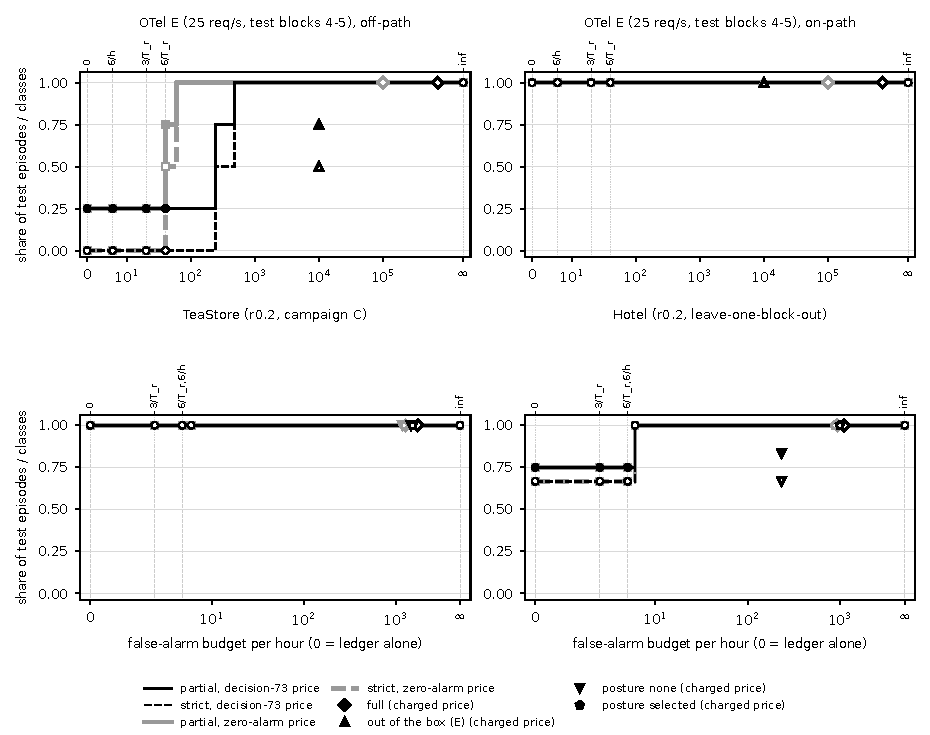
\includegraphics[page=1,trim=0 210.8 214.4 0,clip,width=0.5\textwidth]{figures/fig_sensitivity.pdf}\\
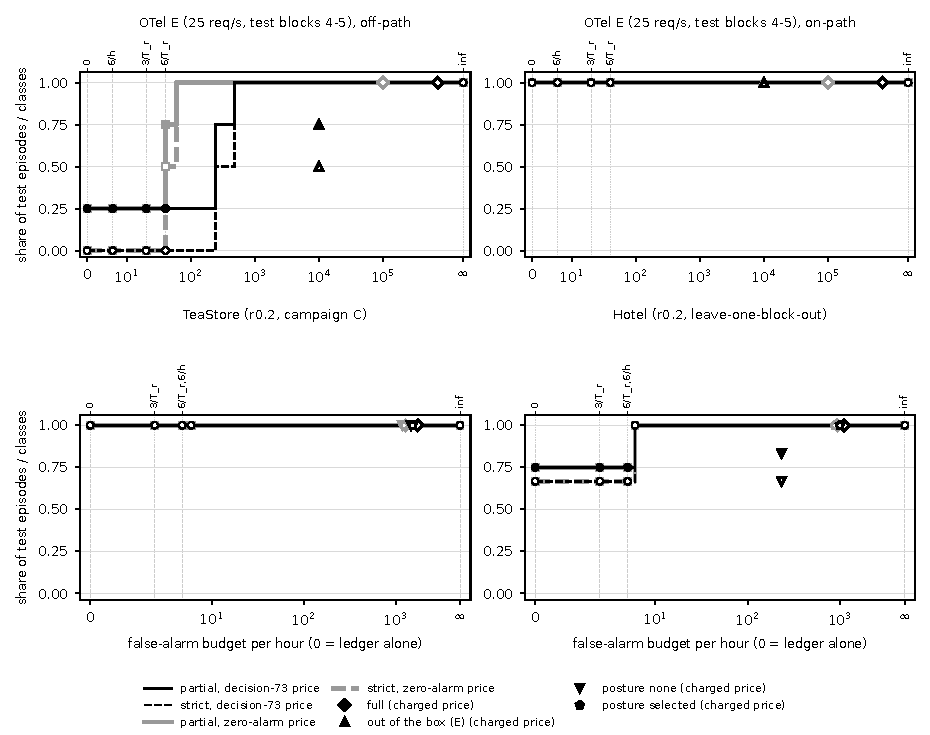
\includegraphics[page=1,trim=78 0 40 320,clip,width=0.6\textwidth]{figures/fig_sensitivity.pdf}
\caption{Post hoc: OTel E off-path test episodes (25\,req/s), detection versus false-alarm budget per hour (0 = ledger
alone). x = the budget $B$ on the CELF set's summed charged training bound (decision 73, or zero-alarm pricing);
comparators at their charged price; not a measured false-alarm rate. Source:
\protect\sid{research/lanes/out-sensitivity-20261014/} (\protect\sid{CURVES.md}; top-left panel and legend of
\protect\sid{fig_sensitivity.pdf} page 1, cropped as recorded in the source comment).}
\label{fig:sens}
\end{figure}
\begin{table}[t]
\caption{Predictions declared before launch, scored on new data (F's 4 off-path test episodes; TeaStore's 10 recommender-pause
episodes per run; Hotel's 20 fault episodes). F's lane rows use the post hoc script frozen before F was read, changed once
after the scorer output was read (recorded deviation, no computation changed). ``BC field'' = by-construction field, not
counted. Sources: the result notes under \protect\sid{research/placement/}; bases and ontology rows in the artifact.}
\label{tab:pred}
\footnotesize
\begin{tabular}{@{}>{\raggedright\arraybackslash}p{1.9cm}>{\raggedright\arraybackslash}p{6.0cm}>{\raggedright\arraybackslash}p{6.8cm}@{}}
\toprule
id, lane & prediction & result \\
\midrule
F-L1 own silence & fire $< 2.0$\,s in 4/4 (BC field) & hit: 0.84--1.52\,s, 4/4 \\
F-L2 coordinator & counted Kafka log fire 42--47\,s in 4/4; none in the 2 frontend episodes & hit: 43.3--44.0\,s, 4/4; none in either frontend episode \\
F-L3 lag & armed, and fires before F-L2 in $\geq 3$/4 & hit: 2 lag ids armed; 4.5--9.3\,s, 4/4 \\
F-M metric arming & $\geq 1$ non-flagd metric placeable & hit: 236 SDK and 44 spanmetrics-derived ids \\
T-L2 coordinator & registry removal line 7.5--12.5\,s in $\geq 9$/10, both rates & hit: 10/10 at 8.37--12.03\,s, all in the BC field \\
T-L1 own silence & recommender CPU down-fire $< 5$\,s in $\geq 9$/10 & miss: 0/10; earliest own fires 14.86--14.92\,s (I/O, CPU pressure) in 5/5 at 10\,req/s, none at 1\,req/s \\
T-OFF off route & login ok $\geq 95$\,\% in $\geq 9$/10; no ledger fire attributable to the pause & miss (read as any counted ledger fire): ok 100\,\% in 10/10; one counted ledger spike (5.07\,s, one episode) \\
T-C control & auth pause detected by the ledger as in C & hit: 10/10 \\
\midrule
\multicolumn{3}{@{}l}{\emph{TeaStore replication 2 and Hotel consul pause; committed \texttt{8b89d43} before replication 2 and the Hotel run launched}} \\
TSR-L2 coordinator & registry removal line 7.5--12.5\,s & hit: 10/10 at 9.09--12.47\,s, all in the BC field \\
TSR, 10 others & own-lane timing, rate dependence, webui line, controls & 9 hits; miss TSR-L1b (own fire at 1\,req/s in 5/5, ceiling 1/5) \\
HO, 4 others & coordinator, search bands, consul own lane, rate ratio (HO-C, L1, L2, D1) & 3 hits (HO-C by construction); miss HO-L2 (own fire 5/10 counted) \\
\bottomrule
\end{tabular}
\end{table}


\subsection{Exploratory (post hoc)}\label{sec:lanes}
Everything in this subsection was computed after the readouts were seen, from the frozen readouts without editing any
frozen file; every set except the frozen ones was chosen in-sample. Over the 175 episodes read before F, the coordinator lane (every log id of
\texttt{kafka} or \texttt{registry}) has a counted hit in 22, a by-construction hit only in 30, no coordinator in 48
(Hotel), a member under degradation without a failure record in 14, a non-member target in 61, and 0 unexplained
\scope{instance}. % POOLED.md Table 2 (first-match failure classes)

\paragraph{Sensitivity curves.}
% research/lanes/out-sensitivity-20261014/CURVES.md (14a72c7); figure = top-left panel and legend of fig_sensitivity.pdf page 1
Figure~\ref{fig:sens} plots partial and strict detection of E's off-path test episodes against the knapsack budget $B$
on the CELF set's summed charged training bound, not a measured false-alarm rate: both reach 1 at 480/h under decision
73 and at 60/h under zero-alarm pricing (grid values). In the source figure's other panels the ledger alone detects
every E on-path and TeaStore C test episode, and Hotel (leave-one-block-out) goes from 0.750 to 1 at 6/h \scope{instance}.


\paragraph{Ontology predictions versus measurement (post hoc).} % research/ontology/runs/run1b-20261014/COMPARISON.md (d943c02); run2-20261014/COMPARISON.md and RUN1B_VS_RUN2.md (d451530)
Over 14 rows \scope{instance} the procedure recovers call graphs and deployment (entry reached as predicted in 11 of 14) but
misses the coordinators: run1b has no OTel coordinator, run2's window of [45, 45]\,s misses the measured 43.3--44.3\,s, and
both runs predict TeaStore's registry lane absent; its lane predictions disagreed with measurement.

\section{Discussion}\label{sec:discussion}

\paragraph{What the protocol changes.} Judged by whether the fault shows up, three of our conclusions would differ.
First, a detection without its price is not a result: with the ledger, the 344 sensors the OpenTelemetry Demo ships detect 3
of 4 off-path test episodes of E at a charged 9,997.39/h \scope{instance}, mostly the zero-alarm floor of 344 sensors
over 0.15\,h; a detection claim should carry its price, bounded by the no-fault
time (Section~\ref{sec:price}) \scope{method}, and appear-only prices are a convention (E's coordinator lane: 366.14/h
charged, 39.94/h at zero alarms). Second, on-path pauses need no placement: the ledger detected every on-path pause episode
(TeaStore's auth and Hotel's search pause at every rate, both OTel frontend-pause test episodes within 0.5\,s)
\scope{cross-sut, three instances}, though not C's 3 throttle episodes at OTel 0.2\,req/s, which nothing detected
\scope{instance}; off path it detected 1 of 4 test episodes in E (3 of 10 over all blocks), 1 of 4 in F, 0 of 4 in the
rerun, the new seed, the fourth run and the TeaStore placement test, while every checkout and login succeeded \scope{instance}.
Third, a sensor can fire on the fault and still be left out of the placement: E's Kafka coordinator log caught 3 of 4 test
episodes at about 44\,s but, never seen in fault-free time, paid the fill price above the budget (Section~\ref{sec:e}),
and E failed; F, with 5\,s export among other changes, passed (a contrast, Section~\ref{sec:f}) \scope{instance}.
% LANES.md O5 (ledger 1/4 test, 3/10 pooled; teastore 7/7, hotel 4/4 per rate); computed here: 344*2.9957/0.15 = 6,870; RESULT_E.md, "Other causes"; RESULT_C.md; RESULT_V2.md; RESULT_TS_OFFPATH.md

\paragraph{Lanes.} Own silence catches every pause episode of the lane tables made before F but reads the injection
back, a ceiling rather than a placement result; it misses Hotel's CPU throttle and the TeaStore recommender pause, and its
median falls with the rate (Hotel: 20.51\,s at 0.05\,req/s, 0.24\,s at 10\,req/s) \scope{instance}. The coordinator lane (post hoc) fired in every pause episode whose target is a coordinator
member and in none other \scope{cross-sut: OTel, TeaStore, pause faults}: Kafka at about 44\,s (session timeout 45\,s),
counted; TeaStore's registry at 8.4--12.5\,s (alive window 10\,s), by-construction field. The lag lane was unarmed in E (113
of 113 matched ids, 60\,s export) and armed in F and its rerun.
% LANES.md O1 (v3.1 rows, prices), O3; RESULT_TS_OFFPATH.md (8.37-12.03 s), RESULT_TS_OFFPATH_REP2.md (9.09-12.47 s); RESULT_F.md

\paragraph{One vocabulary across tools.} Kieker, Jaeger and OpenTelemetry are treated as branded sensors doing the same job:
each contributes identifiers \texttt{channel:service:token}, and alarms come only from that vocabulary (log templates hashed
per line, metric and span names) under five rules fixed in advance and calibrated on fault-free time. The system-specific
signals we found entered as ordinary identifiers, not hand-written alarms: Kafka coordinator log templates, the registry's
heartbeat-removal line, the lag and broker metrics (F) and webui's load-balancer line \scope{instance}; a new system starts from this base and adds only its own
identifiers \scope{method}.

\paragraph{Lessons from building the protocol.} Optimising the placement score is a small part of the protocol; most rules
make the conditions comparable before any score exists (fresh deployments, fault timing bounded by the command, a ledger
independent of instrumentation, calibration on fault-free time only) \scope{method}. Without them a score does not travel:
C's training pattern held at one rate and did not replicate \scope{instance}. One protocol on three stacks (Java with
Kieker, Go with Jaeger, a polyglot OpenTelemetry deployment) required a stack-independent sensor identifier and ledger
\scope{method}. The fault patterns come from chaos practice and the shared-fate hypothesis below from a production
incident review, not from a curated dataset. The model-assisted extraction gathers candidate topology facts from code and
deployment files before any run, but its lane predictions disagreed with measurement, so measurement on the running system
stays the arbiter, offline as here or in an online loop \scope{method}.

\paragraph{Applying it to another system.} A team supplies the system, a workload that replays its usage and the fault
patterns (Table~\ref{tab:task}); the no-fault cells show which services emit what on which channel at that load, to
reconcile with a static extraction (Section~\ref{sec:ontology}) before and after a change \scope{method}.

\paragraph{Shared fate (future work).} A production incident review suggests that a failure's radius depends on where
replicas sit, and that the fastest signal can be a shared layer's silence. % research/PLAN_LANES_20261014.md, "Blast radius and shared-fate groups" (de-identified; this passage is omitted from the artifact copy, REDACTIONS.md)
Placement might then go over shared-fate units first (host, runtime, collector, broker, registry), then signals inside
one \scope{general, hypothesis}; here every telemetry lane shares the collector, and only the ledger is independent of it.

\section{Threats to validity}\label{sec:threats}
\begin{itemize}
\item \emph{Host is confounded with SUT}: one host per SUT (three CPU generations; two of fb14srv6's 24 threads held by
  another user's processes); no number is compared across SUTs. Moving TeaStore from fb14srv5 to fb14srv6 reproduced
  the sign of the first posture step's latency cost but not its size, and detection was not moved. % research/host-topology.json; research/host-rotation/SRV6_RESULT.md
\item \emph{Coverage}: off-path placement was tested on OTel (E failed; F, its rerun, ablation, new seed and a fourth run passed;
  lag chosen in 3 of 4 runs of F's design) and TeaStore (pass at 1\,req/s; at 10\,req/s a fail, then a pass on a repeat), on Hotel only as a negative control.
\item \emph{Few episodes}: 2 test episodes per off-path class and rate in every placement test (a verdict is close to a
  yes/no on one sensor); more runs of one plan, not more episodes per run, are what this paper adds. F's two no-fault cells
  per block are siblings in leave-one-cell-out calibration (optimistic fold estimates); E's 0.15\,h sets the floor 19.97/h;
  fresh false alarms on 0.2\,h per run (floor 14.98/h) can contradict a price but never confirm it. On 0.5\,h of fresh
  no-fault time (post hoc) F's lag sensor stayed below its price (0 alarms); two prices at the zero-alarm floor were neither
  confirmed nor contradicted (4 and 5 alarms) \scope{instance}. % research/placement/test-f-nofault/RESULT_F_NOFAULT.md (9cde956)
\item \emph{Reviews}: every chain and result note had one same-provider adversarial review (Claude subagents;
  log \sid{REVIEWS_LAST_RUNS_20261015.md}); the paper text had cross-provider review by \texttt{gpt-6.1-sol} through an
  LLM-as-judge tool (\sid{REVIEW_JUDGE_20261015.md}), not the result notes; the lane, pooled and curve notes had none.
\item \emph{E and F are not a controlled pair}: they differ in more than the four declared changes (Section~\ref{sec:f});
  F's cadence is partial (one cell: 5\,s for most SDK services, 2\,s flagd, 60\,s frontend, payment, currency); the lag
  sensor sums both groups. % RESULT_F.md
\item \emph{Appear-only pricing}: 3,748 of E's 4,417 candidates (85\,\%) carry the fill price; why they are evaluated in 0
  folds is open. % RESULT_E.md; FREEZE_V33_20261014.md (v3.3 freeze record)
\item \emph{Scoring and fault scope}: sets are scored on \texttt{full}-posture cells (decision 80), so a smaller deployed
  posture, its overhead and its loss of signal are not tested; fresh deployments exclude faults that act through accumulated
  state; doses are a fixed factor (decision 50).
\item \emph{Post hoc material}: the lane, pooled and sensitivity tables and the ontology comparison were made after the
  readouts were seen, their sets in-sample except the frozen ones; T-OFF's script changed once after launch (\texttt{6a42206}, recorded).
\end{itemize}
\section{Artifact}\label{sec:artifact}
The artifact, \url{https://github.com/fhuebscher/PayingAttentiontoSensors}, is a one-commit snapshot with a SHA-256 manifest of every file: the
protocol records (decision log, budgets, declarations, freeze records, timeline, result documents), the analysis code with
registries, split files and tests, the harness code at the launch commits (OTel C \texttt{8018a19}, E \texttt{6a5c2a9}, F
\texttt{715d57b}, ablation \texttt{4ab4433}, new seed \texttt{f08ba1d}; TeaStore C \texttt{3b4a513}, off-path \texttt{f74b29b}
and \texttt{04254228}; Hotel \texttt{9ad0b98}), and the derived readouts, placements, scorer and replay outputs from which
every verdict and table is recomputed (\texttt{uv run pytest -q}). Code is Apache-2.0; data, results and documents are
CC~BY~4.0. Withheld: the raw cell evidence (130\,GB of collector logs, packet captures, container logs and ledgers, which
record lab-host identifiers); the scorers read only the derived readouts. Redactions (a lab domain name, a private incident note,
files with a cloud account identifier) are listed with digests in \texttt{REDACTIONS.md}.
% harness launch commits: DECLARATION_C_OTEL.md (launch log 8018a19), DECLARATION_C_TEASTORE.md, DECLARATION_E_OTEL.md,
% DECLARATION_F_OTEL.md, DECLARATION_F_NOLAG_OTEL.md, DECLARATION_F_OTEL_SEED2.md, DECLARATION_TEASTORE_OFFPATH.md, DECLARATION_TEASTORE_OFFPATH_REP2.md, DECLARATION_HOTEL_OFFPATH.md
% raw evidence size: /usr/bin/du -shc tmp/*-evidence/ = 130 GB over 59 directories (2026-10-15); bundle: tmp/artifact-benchsoc-20261015/

\section*{Declaration on Generative AI}
% Wording follows the CEUR-WS template (template-src/CEURART/sample-1col.tex); content from the author, 2026-10-15 ~13:55Z.
During the preparation of this work, the author used Claude models (Anthropic) in order to: build the experiment tooling;
synchronise scripts to the lab servers and launch and fetch campaigns under the author's authorisation; check the mapping of
campaign results to the declared analyses; and support the writing. An OpenAI model, through an LLM-as-judge tool, gave
cross-provider review. After using these tools, the author reviewed and edited the content as needed and takes full
responsibility for the publication's content.

\bibliography{refs}

\end{document}
